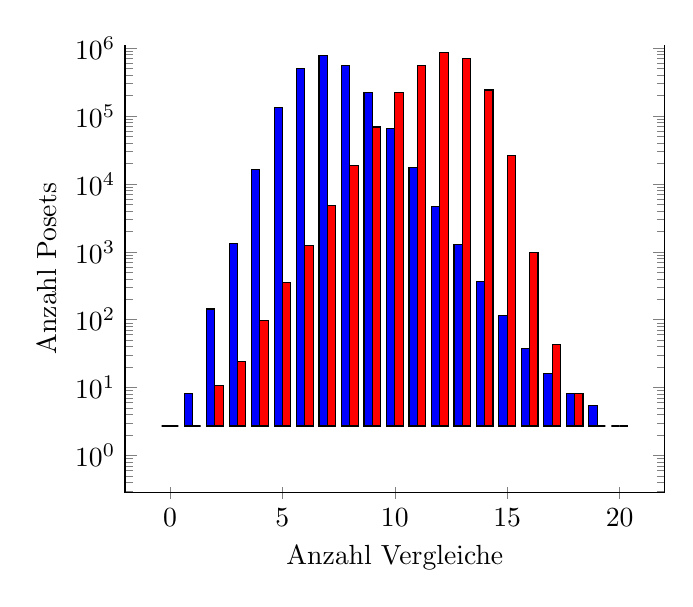
\begin{tikzpicture}
  \begin{axis}[
      ybar,
      ymode=log,
      axis x line = bottom,%x-Achse nur unten
      enlarge x limits = .1,%x-Achse erweitern
      x axis line style = {-},%kein Pfeil
      bar width=3pt,
      ylabel={Anzahl Posets},
      xlabel={Anzahl Vergleiche},
    ]
    \addplot[fill=blue,shift={(1pt, 0)}] table {
        x y
        0 1
        1 3
        2 53
        3 495
        4 5921
        5 49147
        6 182188
        7 283839
        8 207294
        9 81898
        10 23841
        11 6437
        12 1708
        13 477
        14 136
        15 42
        16 14
        17 6
        18 3
        19 2
        20 1
      };
    \addplot[fill=red,shift={(-1pt, 0)}] table { % TODO: update numbers
        x y
        0 1
        1 1
        2 4
        3 9
        4 36
        5 130
        6 461
        7 1770
        8 6848
        9 25372
        10 82456
        11 202924
        12 318522
        13 259021
        14 88920
        15 9509
        16 365
        17 16
        18 3
        19 1
        20 1
      };
  \end{axis}
\end{tikzpicture}